\documentclass[11pt,a4paper,oneside]{report}
\setlength{\textwidth}{6.25in}
\setlength{\textheight}{8in}
\renewcommand{\baselinestretch}{1.3}
\oddsidemargin 20pt
\evensidemargin 20pt
\topmargin 0pt
\newcommand{\squeezeup}{\vspace{-0.6cm}}
\renewcommand*\contentsname{INDEX}
\usepackage{graphicx}
\usepackage{graphics}
\usepackage{listings}
\usepackage{titlesec}
\usepackage{url}
\usepackage{amsmath}
\usepackage{epsfig}
\usepackage{enumerate}
\usepackage[left=3.81cm,top=2.54cm,right=2.54cm,bottom=3.175cm]{geometry}
\usepackage[utf8]{inputenc}
\usepackage[font=normalsize,labelfont=bf]{caption}
\usepackage{xcolor}
\usepackage{pdfpages}
\usepackage{fancyhdr}
\usepackage{float}
\usepackage{fancybox}
\fancypagestyle{plain}

\fancyhf{}
\fancyhead[LE]{\leftmark}
\rhead[RO]{\scriptsize{Synergizing Quantum Computing and Artificial Intelligence: A Review of Trends and Opportunities}}
\cfoot[LE,RO]{\thepage\\\scriptsize{Department of Computer Engineering, GCOERC, Nashik 2025-26}}
\pagestyle{fancy}

\titleformat{\chapter}[display]
{\normalfont\large\bfseries\centering}{\chaptertitlename\ \thechapter}{14pt}{\large}
\titleformat{\section}{\normalsize \bfseries}{\thesection}{1em}{}

\begin{document}
	
	%Title Page
	\begin{titlepage}   
		\thisfancypage{\setlength{\fboxsep}{10pt}\doublebox}{}
		\vspace{0.1in}
		\begin{center}
		{ \bf {A}}\\
		\vspace{0.1in}
		{ \bf {SEMINAR REPORT}}\\
		\vspace{0.1in}
		{ \bf {ON}}\\
		\vspace{0.2in}
		{\Large \bf {``Synergizing Quantum Computing and Artificial Intelligence: A Review of Trends and Opportunities''}}
		\\
		\vspace{0.2in}
		{ SUBMITTED TO THE SAVITRIBAI PHULE PUNE UNIVERSITY}\\
		{ IN PARTIAL FULFILLMENT OF THE REQUIREMENTS}\\
		{ FOR THE AWARD OF THE}\\
		\vspace{0.2in}
		{\bf THIRD YEAR COMPUTER ENGINEERING }\\	
		\vspace{0.1in}
		{\bf BY}\\
		\vspace{0.1in}
		{\bf Mr. Mustafa Murtaza Merchant } \hspace{0.1in}\\ {\small{ (Roll No:  74) }}\\
		
		\vspace{0.2in}
		{\bf UNDER THE GUIDANCE OF}\\
		\vspace{0.1in}
		{\large \bf Mr. Sandeep G. Shukla}\\
		\vspace{0.17in}
		\begin{figure*}[h]
		\centerline{\psfig{figure=./GCOERC.jpg,width=1.8in,height=1.7in}}
		\label{atcres}
		\end{figure*}
		\vspace{0.17in}
		{\large \bf{ DEPARTMENT OF COMPUTER ENGINEERING}}\\ 
		{ \large \bf {Guru Gobind Singh College of Engineering and Research Center, Nashik}}\\ 
		{\bf Khalsa Educational Complex Guru Gobind Singh Marg, Wadala-Pathardi Road, Indira Nagar, Nashik, Maharashtra 422009}\\ 
		\small{YEAR 2025-2026}
		\end{center}
	\end{titlepage}
	%Certificate
	\thisfancypage{\setlength{\fboxsep}{10pt}\doublebox}{}	
	\begin{titlepage}
		\begin{center}
		{\large{ DEPARTMENT OF COMPUTER ENGINEERING}}\\
		{ \large\bf Guru Gobind Singh College of Engineering and Research Center, Nashik}\\ 
		{\bf Khalsa Educational Complex Guru Gobind Singh Marg, Wadala-Pathardi Road, Indira Nagar, Nashik, Maharashtra 422009}\\
		{\bf Year 2025-26}
		\vspace{0.2in}
		\begin{figure*}[!h]
		\centerline{\psfig{figure=./GCOERC.jpg,width=1.5in,height=1.4in}}
		\label{atcres}
		\end{figure*}
		\vspace{0.2in}\\
		{\large\textbf{CERTIFICATE}}\\
		{\small \bf This is to certify that seminar report entitled}\\
		\vspace{0.2in}
		{\large \bf {``Synergizing Quantum Computing and Artificial Intelligence: A Review of Trends and Opportunities''}}\\
		\vspace{0.2in}
		{\small Is submitted as partial fulfilment of \\curriculum of the T.E. Computer Engineering}\\
		\vspace{0.2in}
		BY\\
		\vspace{0.2in}
		{\bf Mr. Mustafa Murtaza Merchant} \hspace{0.1in} \\{\bf (Roll No: 74)}\\
		
		\end{center}
		\vspace*{0.4in}\\
		\hspace{0.2in}(Mr. Sandeep G. Shukla)\hspace{0.2in} (Mr. Ajit R. Pagar)\hspace{0.2in}(Mr.Sandeep. G. Shukla)\\
		\hspace*{0.4in}\bf{Seminar Guide} \hspace*{0.6in}\bf{Seminar Coordinator}\hspace*{0.7in}\bf{Head}\\
		\vspace*{0.2in}\\
		\hspace*{0.4in}Place: {GCOERC, Nashik}\\
		\hspace*{0.4in}Date:
	\end{titlepage}
	%University Certificate
	\thisfancypage{\setlength{\fboxsep}{10pt}\doublebox}{}	
		\vspace{4in}
		\begin{titlepage}				
		\begin{center}	
		{\small Savitribai Phule Pune University}\\
		\begin{figure*}[h]
		\centerline{\psfig{figure=./University.PNG,width=1.8in,height=1.4in}}
		\label{atcres}
		\end{figure*}
		{\large \textbf{CERTIFICATE}}\\
		\vspace{0.2in}
		{\small This is to Certify that}\\
		\vspace{0.2in}
		{\bf Mr. Mustafa Murtaza Merchant} \hspace{0.1in} \\{\bf (Roll No: 74)}\\
		
		\vspace{0.2in}
		{\small Student of T.E. Computer}\\
		{\small was examined in Seminar Report entitled}\\
		\vspace{0.4in}
		{\Large \bf {``Synergizing Quantum Computing and Artificial Intelligence: A Review of Trends and Opportunities"}}\\
		\vspace{0.4in}
		{on $\ldots$/$\ldots$ /2025}\\
		\vspace{0.3in}
		{At}\\
		{ DEPARTMENT OF COMPUTER ENGINEERING,}\\
		{ GURU GOBIND SINGH COLLEGE OF ENGINEERING AND RESEARCH CENTER, NASHIK}\\
		{YEAR 2025-26}\\
		\vspace{0.6in}
		\noindent
		\hspace*{0.3in}$\ldots\ldots\ldots\ldots\ldots\ldots\ldots $\hspace{1.9in} $\ldots\ldots\ldots\ldots\ldots\ldots\ldots $\\
		\hspace*{0.3in} Internal Examiner \hspace*{2.2in} External Examiner\\
		
		\vspace{0.3in}
		\end{center}
	\end{titlepage}
	%Abstract
\addcontentsline{toc}{chapter}{Abstract}
\chapter*{ABSTRACT}
\pagenumbering{roman}
\hspace*{0.3in}
Quantum computing (QC) and artificial intelligence (AI) are coming together in an exciting way, shaking up the tech world, also called as  Quantum Artificial Intelligence (QAI). AI is stepping up to improve how quantum systems are designed, fix errors, and fine-tune algorithms, while QC is turbocharging AI tasks like training machine learning models and tackling tough simulations. In this paper, I dive into how AI is making a difference in QC, think calibrating quantum processors, cutting noise with reinforcement learning, and blending quantum-classical models for big language processing. I also explore some key trends for 2025, the UN’s International Year of Quantum Science and Technology, like scalable error-corrected qubits (check out Google’s Willow chip!), modular setups with over 1,000 qubits, and quantum networks that enable distributed computing.
This paper checks out some really cool real-world uses, like drug research, banking, and cybersecurity, while facing down challenges like qubit decoherence and a real crunch for skilled folks. From what I have found, AI teamed up with quantum computing might just give us a leg up in specialized areas by 2029, unlocking breakthroughs for those tricky problems. But honestly, cracking those scaling issues will take a group effort from all sorts of experts. This study lays out a solid picture for researchers and practitioners, with an eye on the exciting road ahead in this ever-changing field.
\\
\textbf{Keywords: Quantum Computing, Artificial Intelligence, Quantum AI Synergy, Error Correction,
	Reinforcement Learning, Hybrid Models, Qubit Scalability, Quantum Networks, Drug
	Discovery, Financial Optimization, Cybersecurity, Quantum Advantage, NISQ Devices,
	Fault-Tolerant Computing, Machine Learning Acceleration.
}\\
	
% Acknowledgement
\addcontentsline{toc}{chapter}{Acknowledgement}
\chapter*{ACKNOWLEDGEMENT}
\hspace*{0.3in}It is my immense pleasure to work on this seminar {\bf Synergizing Quantum Computing and Artificial Intelligence: A Review of Trends and Opportunities}. It is only the blessing of my divine master which has prompted and mentally equipped me to undergo the study of this seminar. \\
\hspace*{0.3in}I would like to thank {\bf Prof.(Dr). N. G. Nikam}, Principal, Guru Gobind Singh College of Engineering and Research Center for giving me such an opportunity to develop practical knowledge about subject. I am also thankful to {\bf Mr. Sandeep G. Shukla}, Head of Computer Engineering Department for his valuable encouragement at every phase of my seminar work and completion. \\	
\hspace*{0.3in}I offer my sincere thanks to my guide {\bf Mr. Sandeep G. Shukla}, who very affectionately encourages me to work on the subject and gave her valuable guidance time to time. While preparing this seminar I am very much thankful to him. \\
\hspace*{0.3in}I am also grateful to entire staff of Computer Engineering Department for their kind co-operation which helped me in successful completion of seminar.\\

                                                              
\vspace{25mm} 
\begin{flushright}
{
\begin{minipage}{3.5in}
\textbf{Mr. Merchant Mustafa Murtaza}\\

 GCOERC, NASHIK.
\\
\end{minipage}} \hfill
\end{flushright}
	\include{Index}
	\addcontentsline{toc}{chapter}{Index}
	\tableofcontents
	\newpage
	\addcontentsline{toc}{chapter}{List of Figures}
	\listoffigures
	\newpage
	\chapter{INTRODUCTION}\
\pagenumbering{arabic}
\hspace*{0.3in}Today man is able to send and receive any form 
of data may be an e-mail or an audio or video 
just by the click of a button but did he ever 
think how securely his data id being transmitted 
or sent to the other person safely without any 
leakage of information?? The answer lies in 
cyber security. Today Internet is the fastest 
growing infrastructure in every day life. In 
today’s technical environment many latest 
technologies are changing the face of the man 
kind. But due to these emerging technologies 
we are unable to safeguard our private 
information in a very effective way and hence 
these days cyber crimes are increasing day by 
day. Today more than 60 percent of total 
commercial transactions are done online, so this 
field required a high quality of security for 
transparent and best transactions. Hence cyber 
security has become a latest issue. The scope of 
cyber security is not just limited to securing the 
information in IT industry but also to various 
other fields like cyber space etc.
\\

\hspace*{0.3in}Today, almost everybody in the world uses social media
but most of them do not always give concern to security. This
is the procedure of analysis of social media dynamic data to
save from ultimatum in business. Every industry has to face
some sort of a special collection of risks on social. Many put
themselves at the center of controversy or in the press of the
organization. In the present, many people are using social
media in a high percentage. They did not consider their data
and information security. In the present time, Social media
networks are always the main priority target of cyber security
attacks. Because of their massive user base. There are many
studies that explore vulnerabilities of security as well as issues
of privacy in social networking sites. Those researches made
better recommendations to diminish from security risks.
Therefore this analysis focuses mainly on factors of study
impact among users of public sector organizations for the
protection of social media emphasis. Particularly in the
education sector.\\
\hspace*{0.3in}In current times many people are using social media.
Every social media application asking personal details for
signup. Every people give their all details depends with their
privacy without considering whether they are using is more
secure or less secure. Here is the breakdown of personal
information that all social media platforms are gained by
users. Name, email, address book, credit card information,
debit card information, language, etc. There are couple of
tools in security tools. They are social media developers
realized security tools and external web services realized
tools. The combination of those two tools allow for a user to
complete the security of accounts. There are some of them as
an example; two-factor authentication, private account,
security checkup, login notification, password strength
Hiruni Fernando
Department of Information Technology
Sri Lanka Institute of Information Technology
Malabe, Sri Lanka
fernandohiruni55@gmail.com
Shashipraba Perera
Department of Information Technology
Sri Lanka Institute of Information Technology
Malabe, Sri Lanka
shashipraba.56@gmail.com
2
checker, trusted contacts, periodic password changes, external
application or site access checkup, email breaches checkup,
identification code etc\\
\begin{figure}
    \centering
    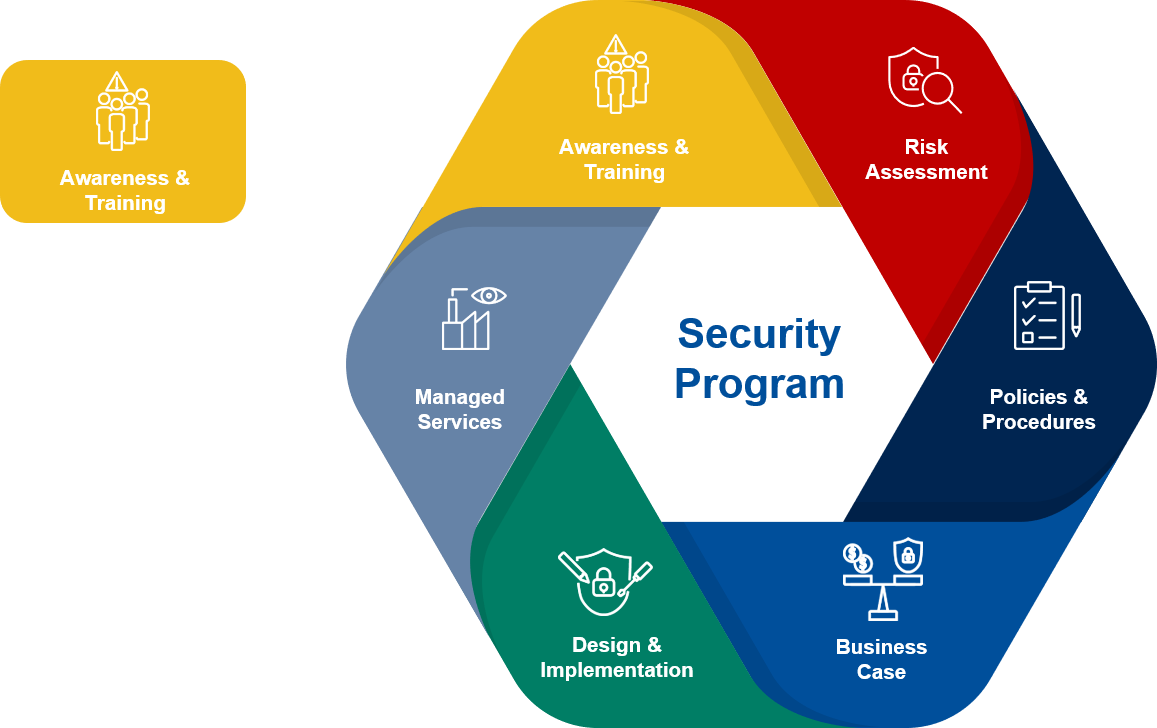
\includegraphics[width=1\linewidth]{AT.png}
    \caption{Security Program}
    \label{fig:enter-label}
\end{figure}
\hspace*{0.3in}Even the latest technologies like cloud 
computing, mobile computing, E-commerce, net 
banking etc also needs high level of security. 
Since these technologies hold some important 
information regarding a person their security 
has become a must thing. Enhancing cyber
security and protecting critical information 
infrastructures are essential to each nation's 
security and economic wellbeing. Making the 
Internet safer (and protecting Internet users) has 
become integral to the development of new 
services as well as governmental policy. The 
fight against cyber crime needs a 
comprehensive and a safer approach. Given that 
technical measures alone cannot prevent any 
crime, it is critical that law enforcement 
agencies are allowed to investigate and 
prosecute cyber crime effectively. Today many 
nations and governments are imposing strict 
laws on cyber securities in order to prevent the 
loss of some important information. Every 
individual must also be trained on this cyber 
security and save themselves from these 
increasing cyber crimes. \\
	
\chapter{HISTORY AND EVOLUTION OF SOCIAL MEDIA}\
\hspace*{0.3in}The use of the internet started to spread and people
experiences new life since 1980 . Social media comprises
communication websites that facilitate relationship forming
between users from diverse backgrounds, resulting in a rich
social structure . More specifically  define social media
as Social media is a means of contact for online interactions
between the end users (viewers) and data generators (data
owners ) who build virtual communities using online social
networks (OSN) .

\\
\hspace*{0.3in}Its being protected by internet-connected systems, including hardware, software and data, from cyber attacks. In a computing context, security comprises cyber security and physical security both are used by enterprises to safe against unauthorized access to data centre and other computerized systems. The security, which is designed to maintain the confidentiality, integrity and availability of data,is a subset of cyber security. \\

\hspace*{0.3in}Historically, organizations and governments have taken a reactive, "point product" approach to combating cyber threats, produce something together individual security technologies - one on top of another to safe their networks andthe valuable data within them. Not only is this method expensive and complex, butnews of damaging cyber breaches continues to dominate headlines, rendering this method ineffective. In fact, given the area of group of people of data breaches, the topic of cyber security has launched to the top of the priority list for boards of directors, which they seeked as far as less risky way. Instead, organizations can a natively integrated, automated Next-Generation Security Platform that is specifically designed to provide consistent, prevention-based protection - on theendpoint, in the data centre, on the network, in public and private clouds, and acrossSaabs environments. By focusing on prevention, organizations can prevent cyber threats from impacting the network in the first place, and less overall cyber securityrisk to a manageable degree \\

\hspace*{0.3in}The Cybersecurity checking began in the 1970s when researcher Bob Thomas created a computer program called Creeper that could move across ARPANET's network. Ray Tomlinson, the innovator of email, wrote the program Reaper, which chased and deleted Creepers. Reaper was the very first example of checking a malware antivirus software and the first self-replicating program i.e. Viruses, as it made first-ever computer worms and trojans.
\\

\hspace*{0.3in} In 1971s, Programmer Bob Thomas made history by innovating a program that is widely accepted as the first incident ever computer trojan as the worm and trojan bounced between computers pc,which has groundbreaker at the time. The trojan was not at all malicious.Manke and Winkler the measures that create the greatest likelihood of security awareness success include the use of creativity in disseminating materials and participatory experiences.

Per NIST 800-50, an awareness program, unlike a security training program, specifically intends to change behavior and culture. It aims to provide information that impacts daily actions. That requires a drastically different approach than just providing information. While employees in some organizations get specific security training, for a vast majority of technology users (common people including college students and school kids), security awareness is limited to some tips for security available in some websites. This is why most security awareness programs fail. The increasing number of data breaches and other cyber-attacks clearly demonstrate that these tips are not enough to raise public security awareness to a level required to create a secure cyber culture.

project and the results of the pilot study that has been done. We have organized the paper in the following way. In next section, we describe related work on this topic. In section 3, we describe the project in details. In section 4 results of the pilot study are discussed. Finally, we draw the conclusion from our study and state our direction for future research on this topic.

    Users exchange a huge amount of personal details on
social networks, making them a target for different types of
Internet attacks, including identity theft, phishing, cyber
bullies, spamming, Web fraud, etc. Social networks provide
hackers with vast opportunities to rob identity. In these types
of attacks, a malicious individual may steal his or her personal
details, including bank accounts, addresses, telephone
numbers, etc., without the user's permission, and using it to
commit cyber-crime. For example, a lot of social networks,
including Facebook, give their users game apps [3]. 

   To complete the registration process, such applications
include personal details, like the user’s credit card details,
phone number, email, etc. Of course, when a user shares the
phone number and credit card details the risk of personal
details theft and phishing attacks is increased. In certain cases,
apps that result in the user resorting to redirect the user's
attention to harmful content and damage its credibility.
   Some of the most obvious potentially innocuous
possibilities in the sense of social networking may be the
illegal use for promotional purposes of personal details, the
collection of possible friends or the discovery of content that
may be of interest. Such techniques are considered a common
process within social networks, and everybody knows about
the collection, review, and usage of personal information for
various purposes, including commercial usage. For one thing,
it has already verified the transfer of personal data from
different social networks.
     One of the main issues for users is that numerous user
specific data leakage can be observed as a consequence of the
social network's failure within the framework of various
initiatives. One causes of significant disruption is hacking user
accounts or lack of accountability, and intercepting all
personal information. When the problem is huge, there will be
more serious issues. There are several possible risks to users,
like computer bugs, malware, Trojan horse, phishing, and
other malicious software, and they can be used to steal
sensitive information from the user.
    According to experts, phishing attacks are one of the most
common cybercrime attacks and the key focus is Internet
payments, Internet banking, Internet stocks, online games,
Web 2.0 technology used pages, and so on [3]. Beyond the
danger of misuse of personal details, social networks are an
instrument for mass demonstrations in the sense of threats to
public security. The disruptive problems of social networks
are revealed to outside intervention, creating tensions between
the government and the people, demonstrations in a short time
\\
	\chapter{LITERATURE SURVEY	}
\hspace*{0.3in}This section consolidates major research contributions in the intersection of Quantum Computing (QC) and Artificial Intelligence (AI), referred to collectively as Quantum Artificial Intelligence (QAI). The works are grouped thematically to highlight foundations, system design strategies, natural language applications, real-world domains, industrial adoption, error correction efforts, and emerging trends.
\section{Quantum AI Foundations And Reviews}
\hspace*{0.3in}Recent surveys highlight how QAI is maturing into a distinct research field. The systematic literature review by Alzubi et al. (2025) synthesizes features and application domains where AI complements QC, ranging from calibration and simulation to optimization tasks [1]. Similarly, a review published in Path of Science (2025) emphasizes algorithmic advances in Quantum Support Vector Machines (QSVM), Quantum Neural Networks (QNN), and Quantum Reinforcement Learning (QRL), positioning them as building blocks of scalable QAI [2]. A broader comprehensive review (2025) situates QML within hybrid computational paradigms, describing transitions from quantum-enhanced classical models to fully native quantum approaches, while addressing challenges of scalability and hybrid integration [3].

\section{AI-Enhanced Quantum System Design And Error Correction}
\hspace*{0.3in}AI has been instrumental in refining quantum hardware control. A study on automatic re-calibration using reinforcement learning demonstrated model-free loops for maintaining stable device performance under drift conditions [4]. Extending this approach, deep reinforcement learning strategies for noise-adaptive qubit routing achieved reductions of up to 37.3\%
 in additional gates and increased success probabilities by 26.8\%
  on noisy devices [5]. Perhaps most notably, Google’s “Willow” processor (2025) introduced a 105-qubit platform that achieved error correction below the surface-code threshold, marking a breakthrough in exponential error suppression and demonstrating the synergy of AI-guided calibration with advanced hardware [6].
\section{Quantum Natural Language Processing (QNLP)}
\hspace*{0.3in}Language processing stands out as a complex yet promising domain. A 2024 survey on QNLP outlines how embeddings, sequential modeling, and attention can be transposed into quantum frameworks, thereby unlocking new pathways for semantic representation [7]. Building on this, the 2025 study on QNLP applications explores distributional compositional categorical models within quantum contexts, offering concrete examples where quantum systems outperform or augment classical NLP in handling ambiguity and compositionality [8].
\begin{figure}[htbp]
	\centering
	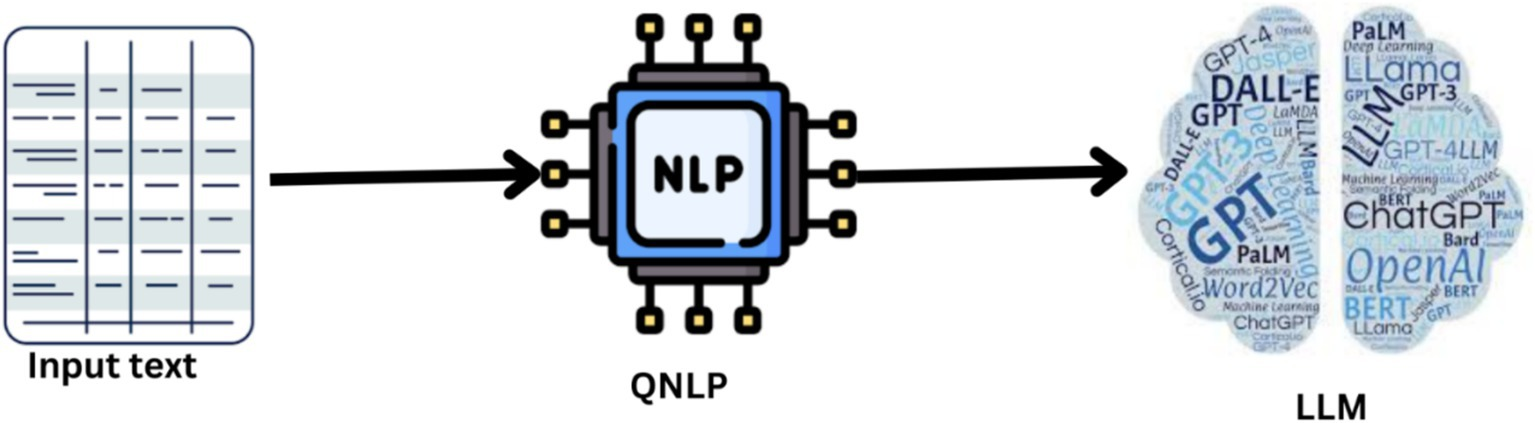
\includegraphics[width=1\linewidth]{qnlp.png}
	\caption{QLM model}
	\label{fig:enter-label}
\end{figure}
\section{Real-World Applications (Drug Discovery, Finance, Healthcare)}
\hspace*{0.3in}Translational impact is increasingly visible across scientific and industrial domains. For example, a study on QML-based electrokinetic mining illustrates how nanoparticles and exosomes can be identified using minimal training data, showcasing QAI’s robustness even in data-scarce biological contexts (citation forthcoming). In drug research, simulations outlined by Quantum Computing Applications: Drug Discovery (2025) highlight how quantum systems accelerate molecular interaction modeling and target discovery cycles [9]. Meanwhile, the QML-based lung cancer prediction framework (2025) demonstrates 85\% classification accuracy with Pegasos QSVC, reflecting QAI’s applicability in Healthcare 4.0 environments [10]. These examples underscore how QAI is evolving from conceptual frameworks into practical solutions.
\section{Quantum AI in Industry \& Business Intelligence}
\hspace*{0.3in}Industrial transformation is exemplified by research on Quantum AI-driven business intelligence for carbon-neutral supply chains. Here, QAI integrates predictive analytics with autonomous decision-making, enabling organizations to optimize logistics, lower carbon footprints, and enhance sustainability reporting [11]. This marks a key step toward embedding QAI into enterprise-scale workflows.
\section{Error Correction \& Noise Mitigation}
\hspace*{0.3in}Error correction remains a central bottleneck in quantum computing. A Nature publication (2024) demonstrated surface-code memories at distance-5 and distance-7, pushing error rates below threshold and confirming fault-tolerant viability [12]. Complementarily, epistemological work on non-classical logic frameworks achieved a 38\% improvement in quantum state representation accuracy, suggesting that theoretical perspectives on knowledge representation are equally crucial for advancing error mitigation [13].
\section{Emerging Trends \& Forecasts}
\hspace*{0.3in}Looking ahead, the McKinsey Quantum Technology Monitor (2025) projects market revenues of up to \$97 billion by 2035, underscoring the momentum in quantum computing, sensing, and communication [14]. Similarly, “Quantum Artificial Intelligence: Unleashing the Next Frontier” (2025) identifies near-term opportunities in drug discovery, financial optimization, and control systems, while stressing the need for scalable architectures [15]. These forward-looking studies converge on a timeline where QAI is expected to transition from experimental proofs to mainstream applications by 2029.
\begin{figure}[htbp]
	\centering
	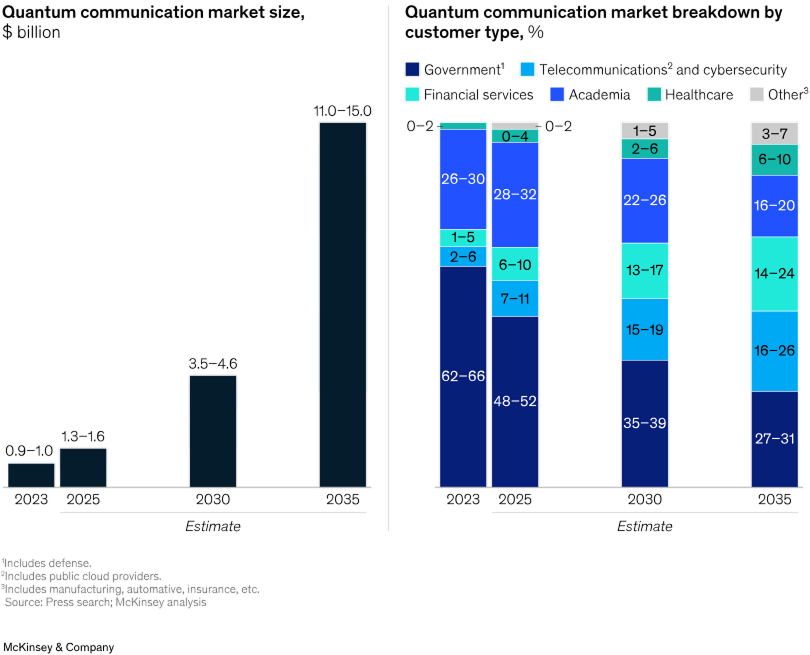
\includegraphics[width=0.9\linewidth]{qt351.png}
	\caption{Quantum Communication market size projectionby 2035}
	\label{fig:enter-label}
\end{figure}
	\chapter{AI-ASSISTED QUANTUM SYSTEM DESIGN \& CONTROL}
\hspace*{0.3in}Artificial Intelligence (AI) is playing an increasingly critical role in the optimization and stability of quantum computing systems. The delicate nature of qubits—susceptible to noise, drift, and hardware imperfections—demands continuous calibration and intelligent control strategies. AI-driven methods, particularly reinforcement learning (RL), have shown promise in addressing these challenges in ways that scale beyond traditional manual approaches.
\section{AI for Calibration, Pulse Shaping, and Continuous Recalibration}
\hspace*{0.3in}Quantum devices require precise control over gate operations and qubit interactions. Conventional calibration procedures, often manual and time-consuming, become impractical as qubit counts scale. AI-based approaches automate these processes by learning the relationships between control parameters and system performance. For example, reinforcement learning agents can optimize pulse sequences to minimize error rates while adapting dynamically to hardware drift. Continuous recalibration ensures that quantum processors remain operationally stable during extended computations, reducing downtime and increasing fidelity.
\section{RL and Model-Free Control Loops (Practical Examples)}
\hspace*{0.3in}Model-free RL techniques are particularly valuable in scenarios where physical models of noise and hardware imperfections are incomplete. Recent studies demonstrate how RL agents can iteratively adjust gate parameters without explicit knowledge of the underlying system [4]. In practice, this allows devices to autonomously maintain performance, even in environments where fluctuations occur unpredictably. Such closed-loop learning reduces the reliance on human expertise and paves the way for “self-healing” quantum hardware.
\section{Qubit Routing, Compilation-Aware Optimization}
\hspace*{0.3in}As quantum algorithms are mapped onto hardware, qubits must often be swapped or routed due to limited connectivity in quantum processors. This introduces additional gates, which amplify error rates. AI-assisted compilation tools—leveraging deep reinforcement learning—can generate noise-adaptive routing strategies, cutting down on unnecessary operations and improving overall success probability [5]. By combining hardware-aware compilation with real-time calibration, these approaches enhance the efficiency of near-term quantum devices and bring hybrid quantum-classical workflows closer to practical deployment.

	\chapter{ ROLE OF CYBER SECURITY IN SOCIAL MEDIA  
}
\hspace*{0.3in}As we become more social in an increasingly 
connected world, companies must find new 
ways to protect personal information. Social 
media plays a huge role in cyber security and 
will contribute a lot to personal cyber threats. 
Social media adoption among personnel is 
skyrocketing and so is the threat of attack. Since 
social media or social networking sites are 
almost used by most of them every day it has 
become a huge platform for the cyber criminals 
for hacking private information and stealing 
valuable data. 
\\
\hspace*{0.3in}In a world where we’re quick to give up our 
personal information, companies have to ensure 
they’re just as quick in identifying threats, 
responding in real time, and avoiding a breach 
of any kind. Since people are easily attracted by 
these social media the hackers use them as a bait 
to get the information and the data they require. 
Hence people must take appropriate measures 
especially in dealing with social media in order 
to prevent the loss of their information.
The ability of individuals to share information 
with an audience of millions is at the heart of the 
particular challenge that social media presents to 
businesses. In addition to giving anyone the 
power to disseminate commercially sensitive 
information, social media also gives the same 
power to spread false information, which can be 
just being as damaging. The rapid spread of 
false information through social media is among 
the emerging risks identified in Global Risks 
2013 report.\\

\hspace*{0.3in}Though social media can be used for cyber 
crimes these companies cannot afford to stop 
using social media as it plays an important role 
in publicity of a company. Instead, they must 
have solutions that will notify them of the threat 
in order to fix it before any real damage is done.
However companies should understand this and 
recognise the importance of analysing the 
information especially in social conversations 
and provide appropriate security solutions in 
order to stay away from risks. One must handle 
social media by using certain policies and right 
technologies.\\
\section{Cyber Crime}
\hspace{0.3in}Cyber crime is a term for any illegal activity that 
uses a computer as its primary means of 
commission and theft. The U.S. Department of 
Justice expands the definition of cyber crime to 
include any illegal activity that uses a computer 
for the storage of evidence. The growing list of 
cyber crimes includes crimes that have been 
made possible by computers, such as network 
intrusions and the dissemination of computer 
viruses, as well as computer-based variations of 
existing crimes, such as identity 
theft, stalking, bullying and terrorism which 
have become as major problem to people and 
nations. Usually in common man’s language 
cyber crime may be defined as crime committed 
using a computer and the internet to steel a 
person’s identity or sell contraband or stalk 
victims or disrupt operations with malevolent 
programs. As day by day technology is playing 
in major role in a person’s life the cyber crimes 
also will increase along with the technological 
advances
\\


	\chapter{QUANTUM NATURAL LANGUAGE PROCESSING (QNLP)}
\hspace*{0.3in}Quantum Natural Language Processing (QNLP) is an emerging area of Quantum Artificial Intelligence that explores how quantum mechanics can enhance the way machines understand and process human language. Three main paradigms dominate current research: distributional models, which represent word meanings as high-dimensional vectors encoded in quantum states; compositional models, such as the distributional compositional categorical (DisCoCat) framework, which map grammatical structures into quantum circuits for syntactic-semantic alignment; and hybrid models that integrate classical NLP with quantum subroutines to balance scalability with near-term quantum hardware constraints. Early applications of QNLP include semantic similarity detection, question answering, and low-resource machine translation, where the parallelism of quantum states provides richer contextual representations [7].\\
\begin{figure}[htbp]
	\centering
	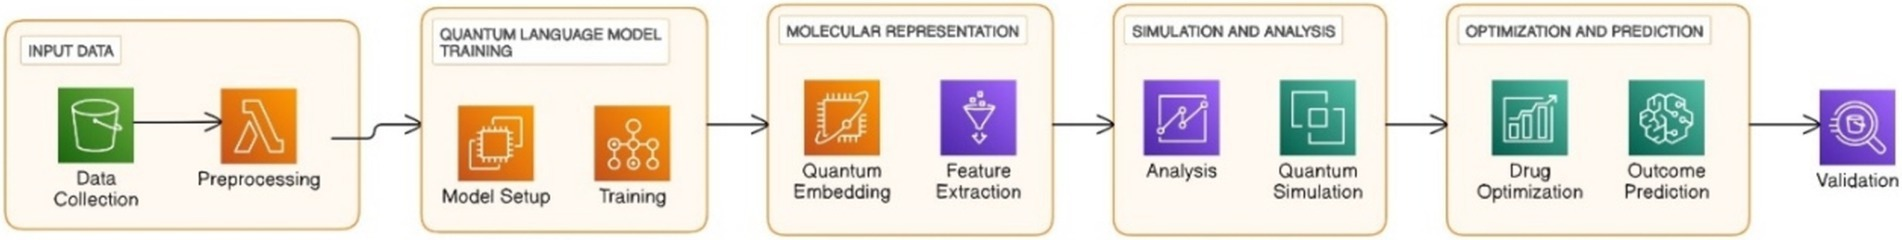
\includegraphics[width=1\linewidth]{qnlpD.jpg}
	\caption{QNLP drug discovery and design.}
	\label{fig:enter-label}
\end{figure}
\\
\begin{figure}[htbp]
	\centering
	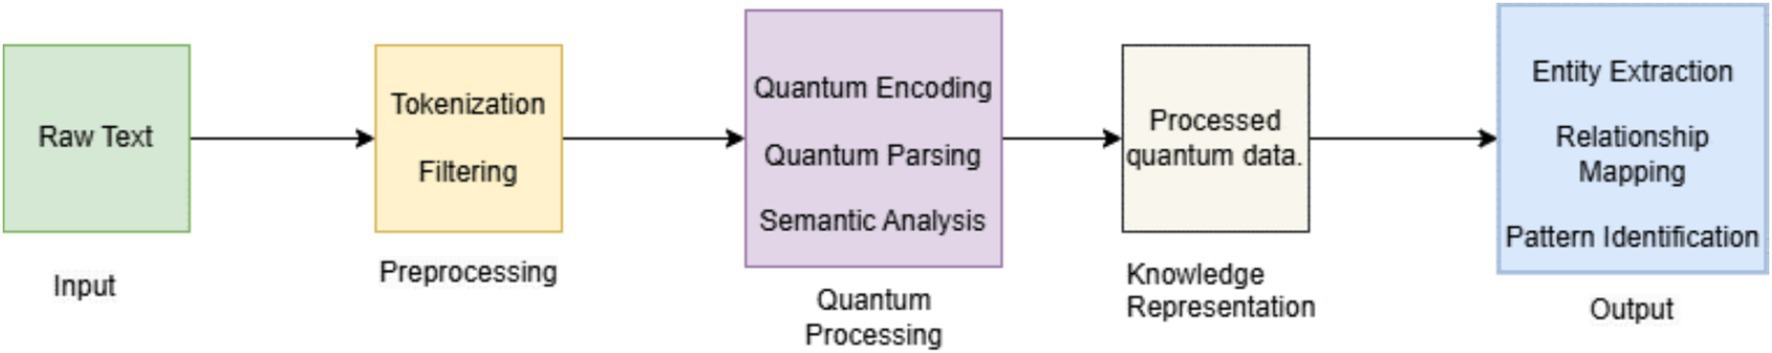
\includegraphics[width=1\linewidth]{qnlpG.jpg}
	\caption{QNLP literature mining and knowledge extraction.}
	\label{fig:enter-label}
\end{figure}
\\
\hspace*{0.3in}Despite this promise, today’s noisy intermediate-scale quantum (NISQ) devices face major limitations, including noise, decoherence, and limited qubit counts, restricting QNLP to smaller tasks rather than large-language-model (LLM)-scale workloads. The roadmap toward practical QNLP requires algorithmic innovation in quantum embeddings and DisCoCat circuits, hardware advances in error-corrected and modular qubits, and hybrid integration where quantum accelerates specific language subtasks while classical systems manage scale. By 2029, QNLP is expected to serve as a complementary layer to classical LLMs, augmenting semantic reasoning, disambiguation, and symbolic integration rather than replacing established large-scale models [8].

	\chapter{CONCLUSION}

\hspace*{0.3in} social
media includes high-security risks as well as risks to privacy.
Because of their centralized infrastructure, their massive
archive of all the personally identifiable data a hacker could
ever need, and the general public’s ignorance of how to
properly use privacy settings to improve their online security
[9], they run this danger. There is also a huge danger, because
a lot of people, especially adolescents, always tend to trust
other people quickly. So, they become extremely confident
about others. Not only that they also share private details about
themselves without a proper understanding of what kind of
details they should share about themselves online.

   Social media have some benefits, but in addition to these
advantages, OSN's posed some similar concerns. Users'
privacy and protection, and their information, are key issues
in social media [4]. While there is some general opinion about
what social media security and what it can help the online
users, there are still many unanswered questions. We think
that the headway of new technology as a rule and specifically,
social sites will bring new security risks which may open the
doors to vindictive performers, key lumberjacks, Trojan
horses, phishing, spies, viruses and attackers [6]. However,
there are many possible solutions presented to avoid the risks.
Information security experts, government officials, and other
intelligence officers need to develop new strategies that
combat and adjust to the emerging future risks and threats [6].
Moreover in the technical aspect, for preserving the security
of social media, techniques like K-anonymity and diversity
can be used\\




	\chapter{QUANTUM NATURAL LANGUAGE PROCESSING (QNLP)}
\section{2025 Milestones}
\hspace*{0.3in}The year 2025, declared the International Year of Quantum Science and Technology, marks a turning point in quantum research and industry adoption. According to the McKinsey Quantum Technology Monitor (2025), global investments and strategic partnerships have accelerated, with projected revenues of up to \$97 billion by 2035 [14]. Breakthroughs such as Google’s Willow processor achieving scalable error correction below threshold [6], and the development of modular architectures exceeding 1,000 qubits, signal that the field is moving from proof-of-concept devices to commercially viable platforms. Quantum networks and early prototypes of distributed computing systems further underscore the progress toward practical large-scale quantum ecosystems.
\section{Near-Term Advantages for QAI (2025–2029)}
\hspace*{0.3in}Quantum Artificial Intelligence (QAI) is expected to deliver measurable benefits in highly specialized domains well before universal fault-tolerant quantum computers arrive. Areas such as drug discovery, financial risk optimization, and cybersecurity anomaly detection are likely to benefit most, due to their reliance on complex optimization and simulation tasks that hybrid quantum-classical approaches can already enhance [9][10][15]. Similarly, Quantum Natural Language Processing (QNLP) is poised to impact data-intensive tasks like semantic search and domain-specific information retrieval [7][8]. Between 2025 and 2029, hybrid architectures that leverage classical AI for stability and scalability, combined with quantum subroutines for exponential speedups in sub-tasks, will remain the dominant mode of deployment.
\section{Research \& Collaboration Priorities}
\hspace*{0.3in}To unlock the potential of QAI, multidisciplinary collaboration is essential. Key priorities include:
\begin{itemize}
	\item \textbf{Scalable error-corrected architectures}: advancing modular qubit systems and efficient error suppression techniques [12].
	\item \textbf{Hybrid AI-quantum frameworks:} integrating reinforcement learning and optimization into quantum workflows to improve system adaptability [4][5].
	\item \textbf{Standardization \& benchmarking:} developing open benchmarks for QML algorithms to ensure comparability and reproducibility across platforms.
	\item \textbf{Talent development \& policy:} addressing the skills gap by fostering programs that merge AI, quantum physics, and systems engineering.
\end{itemize}
	\chapter{CONCLUSION}
\hspace*{0.3in}This review highlighted how Quantum Computing (QC) and Artificial Intelligence (AI) are converging to form Quantum Artificial Intelligence (QAI), a field with the potential to reshape computation. AI is accelerating progress in quantum hardware calibration, error correction, and algorithm design, while quantum systems are showing promise in enhancing machine learning tasks such as optimization, simulation, and natural language processing. Real-world applications in healthcare, drug discovery, finance, and business intelligence demonstrate that QAI is moving beyond theory into practical domains, though challenges like decoherence, scalability, and workforce shortages remain significant.\\

\hspace*{0.3in}Looking forward, the next decade will be critical in transforming proofs-of-concept into scalable systems. Future research should focus on achieving robust error correction, developing hybrid frameworks that balance classical and quantum resources, and addressing ethical implications of QAI deployment. Interdisciplinary collaboration and global cooperation will be essential to overcome technical and societal barriers, ensuring that QAI becomes not just a specialized research area but a cornerstone of 21st-century innovation.\\
	\include{conclusion}
	
	\footnotesize
	\addcontentsline{toc}{chapter}{REFERENCES}
	\renewcommand\bibname{References}
	\begin{thebibliography}{}
		\item[1] Vanessa García Pineda, Alejandro Valencia-Arias, Francisco Eugenio López Giraldo, Edison Andrés Zapata-Ochoa, "Integrating Artificial Intelligence and Quantum Computing: A Systematic Literature Review of Features and Applications," 2025. [Online]. Available: https://www.sciencedirect.com/science/article/pii/S266630742500035X.  
		
		\item[2] Ololade Funke Olaitan, Samuel Oluwabukunmi Ayeni, Adedapo Olosunde, Francis Chukwudalu Okeke, Ugochukwu Udonna Okonkwo, Chukwuemeka George Ochieze, Osinachi Victor Chukwujama, Ogheneruemu Nathaniel Akatakpo, "Quantum Computing and Artificial Intelligence: A Review of Quantum Machine Learning Algorithms," Path of Science, vol. 10, no. 6, 2024. [Online]. Available: https://pathofscience.org/index.php/ps/article/view/3541.  
		
		\item[3] Devadas RM, T S., "Quantum Machine Learning: A Comprehensive Review of Integrating AI with Quantum Computing for Computational Advancements," Journal of Computational Science, 2024. [Online]. Available: https://pubmed.ncbi.nlm.nih.gov/40331033/.  
		
		\item[4] T. Crosta, L. Rebón, F. Vilariño, J. M. Matera, M. Bilkis, "Automatic Re-calibration of Quantum Devices by Reinforcement Learning," 2024. [Online]. Available: https://arxiv.org/abs/2404.10726.  
		
		\item[5] G. Pascoal, J. P. Fernandes and R. Abreu, "Deep Reinforcement Learning Strategies for Noise-Adaptive Qubit Routing," IEEE Transactions on Quantum Engineering, 2024. [Online]. Available: https://ieeexplore.ieee.org/document/10646540/.  
		
		\item[6] Jin, Yirong, "Google's 'Willow' Quantum Processor: New RCS Record, and First Error Correction Below the Surface Code Threshold," Quantum, vol. 9, 2025. [Online]. Available: https://linkinghub.elsevier.com/retrieve/pii/S2666675825001456.  
		
		\item[7] Dominic Widdows, Willie Aboumrad, Dohun Kim, Sayonee Ray, Jonathan Mei, "Natural Language, AI, and Quantum Computing in 2024: Research Ingredients and Directions in QNLP," 2024. [Online]. Available: https://arxiv.org/abs/2403.19758.  
		
		\item[8] Pallavi Gundala, Prasanna Kumar Rangarajan, "Quantum Natural Language Processing and Its Applications," Frontiers in Computer Science, 2025. [Online]. Available: https://www.frontiersin.org/journals/computer-science/articles/10.3389/fcomp.2025.1464122/full.  
		
		\item[9] Quantum News, "Quantum Computing Applications: Drug Discovery," Quantum Zeitgeist, 2024. [Online]. Available: https://quantumzeitgeist.com/quantum-computing-applications-drug-discovery/.  
		
		\item[10] M. Munshi, R. Gupta, N. K. Jadav, S. Tanwar, A. Nair and D. Garg, "Quantum Machine Learning-Based Lung Cancer Prediction Framework for Healthcare 4.0," IEEE Access, 2024. [Online]. Available: https://ieeexplore.ieee.org/document/10673456/.  
		
		\item[11] Sanjai Vudugula, Sanath Kumar Chebrolu, "Quantum AI-Driven Business Intelligence for Carbon-Neutral Supply Chains," African Journal of Advanced Technology and Engineering Studies, vol. 2, no. 1, 2024. [Online]. Available: https://ajates-scholarly.com/index.php/ajates/article/view/16.  
		
		\item[12] Google Quantum AI and Collaborators, "Quantum Error Correction Below the Surface Code Threshold," Nature, vol. 631, no. 8021, 2024. [Online]. Available: https://www.nature.com/articles/s41586-024-08449-y.  
		
		\item[13] Fasco , Pamba Shatson, "Beyond Boolean Epistemology: A Non-Classical Logic Approach to Understanding Knowledge Formation in Quantum Computing Systems," International Journal of Scientific Research and Management, vol. 12, no. 8, 2024. [Online]. Available: https://ijsrm.net/index.php/ijsrm/article/view/6089.  
		
		\item[14] McKinsey \& Company, "The Year of Quantum: From Concept to Reality in 2025," 2025. [Online]. Available: https://www.mckinsey.com/capabilities/mckinsey-digital/our-insights/the-year-of-quantum-from-concept-to-reality-in-2025.  
		
		\item[15] SpinQ Team, "Quantum Artificial Intelligence: Unleashing the Next Frontier in Computing," SpinQuanta News, 2024. [Online]. Available: https://www.spinquanta.com/news-detail/quantum-artificial-intelligence-unleashing-the-next-frontier-in-computing-with-spinq.  
	\end{thebibliography}
	
\end{document}